\documentclass[xcolor={dvipsnames}]{beamer}
\usetheme{Malmoe}
\usecolortheme{spruce}
\setbeamercolor{item}{fg=PineGreen}
\setbeamertemplate{itemize item}[square]
\setbeamertemplate{itemize subitem}[triangle]
\setbeamertemplate{itemize subsubitem}[square]
\setbeamertemplate{itemize/enumerate subbody begin}{\vspace{0.5em}}

\usepackage{amsmath,amsthm,amssymb}
\usepackage{mathtools}
\usepackage{mathrsfs}
\usepackage{physics}
\usepackage{graphicx}
\usepackage{caption}
\usepackage{algpseudocode, algorithm}
\usepackage{animate}

\captionsetup[figure]{labelformat=empty}
\graphicspath{ {./images/} }

\let\olditemize=\itemize 
\let\endolditemize=\enditemize 
\renewenvironment{itemize}{\olditemize \itemsep=.5em }{\endolditemize}

\newcommand{\ord}[1]{\mathcal{O}(#1)}

\title{Complexity of Jet Reconstruction Algorithms}
\author{Sean Ericson}
\institute{UO\\PHYS 662}
\date{March 18, 2024}
\titlegraphic{
\includegraphics[scale=0.7]{seal.jpg}}

\begin{document}

\frame{\titlepage}

\begin{frame}{Complexity of Jet Algorithms}
\begin{itemize}
    \item<1-> Jet Reconstruction algorithms are at the core of modern HEP data collection and analysis
    \item<2-> Efficient algorithms are necessary to make analysis of large datasets feasible.
    \item<3-> Outline
    \begin{itemize}
        \item<5-> Review of jet algorithms
        \item<6-> Measuring Algorithmic Complexity
        \item<7-> Analysis of FastJet, SISCone, and their predecessors
    \end{itemize}
\end{itemize}
\end{frame}

\begin{frame}{Review of Jet Algorithms}
\begin{itemize}
    \item<1-> Jet algorithm goals:
    \begin{itemize}
        \item<2-> Combine data from calorimeters and trackers to define jets
        \item<3-> Identify subjets and jet substructure
        \item<4-> Measure invariant masses of constituent particles
        \item<5-> Identify missing energy/momentum
    \end{itemize}
    \item<6-> Jets:
    \begin{itemize}
        \item<7-> A collimated spray of stable particles arising from fragmentation and hadronization of a parton after a collision.
    \end{itemize}
\end{itemize}
\end{frame}

\begin{frame}{Review of Jet Algorithms (cont.)}
\begin{figure}
    \centering
    \captionof{figure}{Example Jet}
    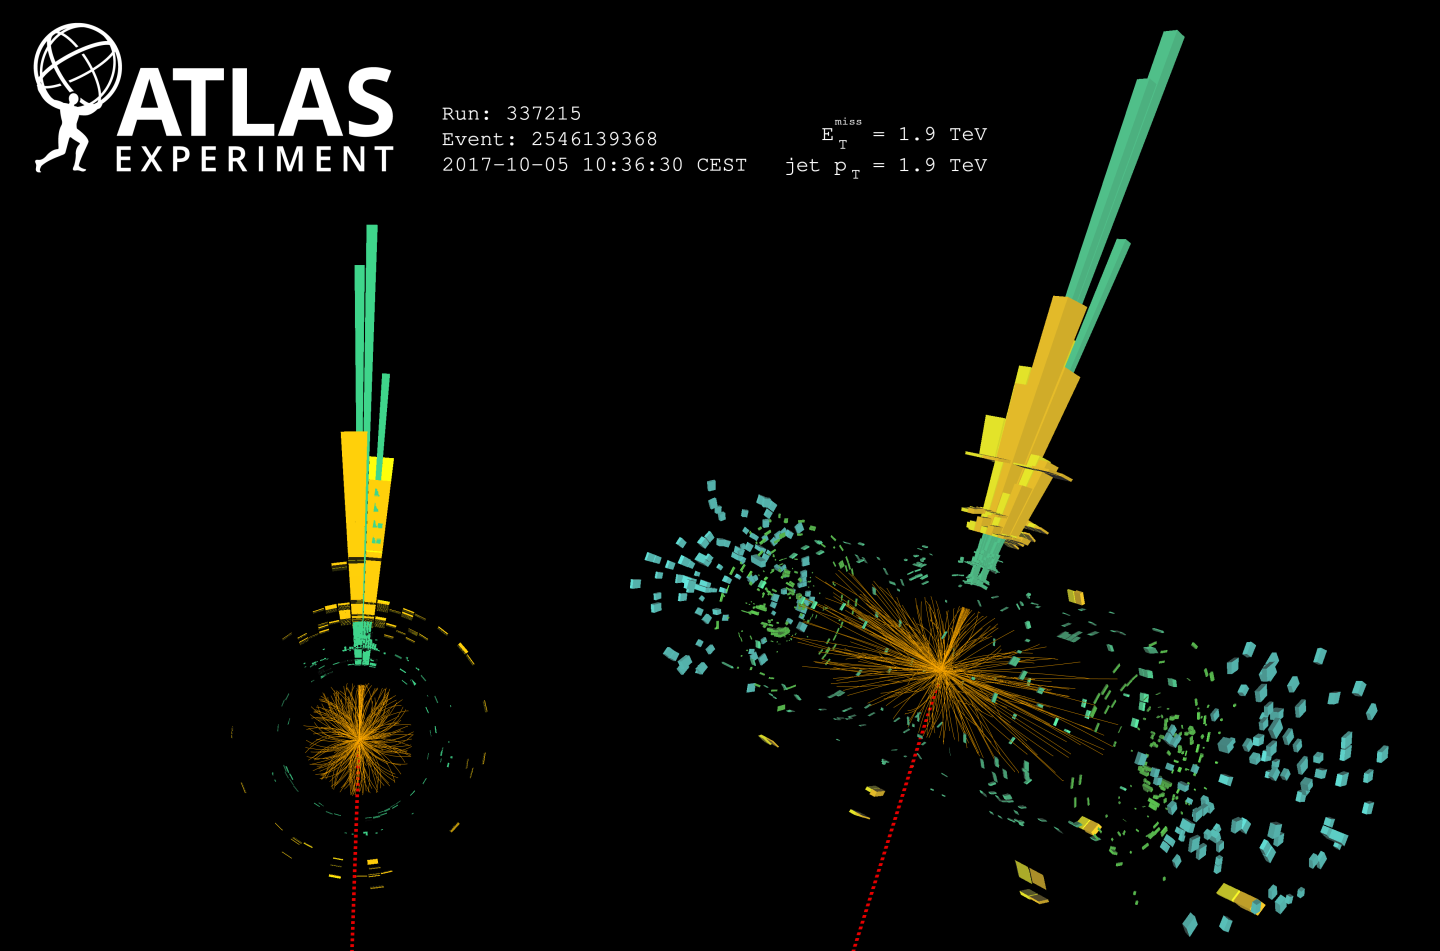
\includegraphics[scale=0.27]{jet_example.png}
\end{figure}
\end{frame}

\begin{frame}{Review of Jet Algorithms (cont.)}
\alert{Considerations}
\begin{itemize}
    \item<2-> Jet size
    \begin{itemize}
        \item<3-> Must be large enough to capture all particles for correct $p_\mu$ calculation.
        \item<4-> However, larger jets are more susceptible to underlying events (UE) and pileup (PU)
    \end{itemize}
    \item<5-> Jet shape
    \begin{itemize}
        \item<6-> Algs with variable jet shape can allow for good resolution of subjets at the expense of greater susceptibility to UE and PU
    \end{itemize}
    \item<7-> Infrared and Collinear safety (IRC safety)
    \begin{itemize}
        \item<8-> Calculated jets should be insensitive to emission of soft radiation from, or collinear splitting of the constituent particles.
        \item<9-> Necessary for faithful comparison of data to experiment
    \end{itemize}
\end{itemize}
\end{frame}

\begin{frame}{Review of Jet Algorithms (cont.)}
\alert{Class of Jet Algorithms}
\begin{itemize}
    \item<2-> Cone Algorithms
    \begin{itemize}
        \item<3-> Assume particles in jets will appear in conical regions; cluster in $(\eta, \phi)$-space.
        \item<4-> Easy to implement, but typically contain unphysical parameters which hinder analysis
        \item<5-> Most are not IRC safe
        \item<6-> Examples include IC-PR, IC-SM, and SISCone.
    \end{itemize}
    \item<7-> Sequential Clustering Algorithms
    \begin{itemize}
        \item<8-> Assume particles in jets have small differences in $p_t$; cluster in momentum space.
        \item<9-> Automatically IRC safe
        \item<10-> Examples include $K_t$, $\bar{K}_t$, and Cambridge/Aachen
    \end{itemize}
\end{itemize}
\end{frame}

\begin{frame}{Measuring Algorithmic Complexity}
\alert{Assymptotics and Big-O Notation}
\begin{itemize}
    \item<2-> Algorithm runtime depends on the specific hardware its running on, and on the input to the particular problem instance
    \item<3-> How can we compare algorithms in a context-independent way?
    \begin{itemize}
        \item<4-> Big-O Notation! (a.k.a Bachmann-Landau/asymptotic notation)
        \item<5->[] $f(x) \in \ord{g(x)}_{x\to\inf} \iff \exists c\; \exists x_0\; \forall x>x_0:\; \abs{f(x)} \leq cg(x)$
        \item<6-> E.g. $\ord{\ln(x)} \subset \ord{x} \subset \ord{x^n} \subset \ord{e^x} \subset \ord{x!}$
        \item<7-> Also, $o()$, $\Theta(x)$, $\Omega()$, $\omega()$ with related definitions
    \end{itemize}
    
\end{itemize}
\end{frame}

\begin{frame}{Complexity of $K_t$ (pre-FastJet)}
\alert{The Naïve Algorithm}
\begin{algorithm}[H]
    \caption{Naïve $K_t$}
    \begin{algorithmic}[1]
        \Repeat
            \For{particle pair $(i,j)$}
                \State $d_{Bi} \gets p_{ti}^2$ \Comment{Calculated once for each $i$}
                \State $R_{ij}^2 \gets (\eta_i - \eta_j)^2  + (\phi_i - \phi_j)^2$ 
                \State $d_{ij} \gets \min(p_{ti}^2, p_{tj}^2)R_{ij}$
            \EndFor
            \State $d_\text{min} \gets \min(\{d_{ij}\}\cup\{d_{Bi}\})$
            \If{$d_\text{min}$ is $d_{Bi}$}
                \State Add particle $i$ to list of jets, remove from list of particles
            \Else{}
                \State Merge particles $i, j$
            \EndIf
        \Until{no particles remain}
    \end{algorithmic}
\end{algorithm}
\end{frame}

\begin{frame}{Pre-FastJet $K_t$ Complexity (cont.)}
\alert{Complexity Analysis}
\begin{itemize}
    \item<2-> Outermost loop executes $\mathcal{O}(n)$ times
    \begin{itemize}
        \item<3-> Calculation of $d_{Bi}$ initially $\ord{N}$, updates actually $\ord{1}$
        \item<4-> Calculation of $d_{ij}$ initially $\ord{N^2}$, updates actually $\ord{N}$
        \item<5-> Determining $d_\text{min}$ is $\ord{N^2}$
        \item<6-> Merging operation is $\ord{1}$
    \end{itemize}
    \item<7-> Full time complexity is therefore \[ \ord{N + N^2 + N(1 + N + N^2 + 1)} = \ord{N^3} \]
    \item<8-> Also easy to see that the space complexity is $\ord{N^2}$.
\end{itemize}
\end{frame}

\begin{frame}{Enter: FastJet}
\alert{Geometric Insight}
\begin{itemize}
    \item<2-> The key to improving $K_t$ is the (rather obvious) geometric insight:
    \begin{itemize}
        \item<3-> Let $d_\text{min} = \min(\{d_{ij}\})$, and let $p_{ti} < p_{tj}$.
        \item<4-> Then, $\forall l:\;R_{ij} \leq R_{il} \quad$
    \end{itemize}
    \item<5-> That is, particles $i$ and $j$ are geometric \textit{nearest neighbors}
    \item<6-> Therefore, we don't need the $\ord{N^2}$ table $d_{ij}$!
    \item<7-> We only need an $n$-element list of nearest neighbors $d_{i\mathcal{G}_i}$
\end{itemize}
\end{frame}

\begin{frame}{Complexity of FastJet}
\alert{The Smart Algorithm}
\begin{algorithm}[H]
    \caption{\texttt{FastJet} $K_t$}
    \begin{algorithmic}[1]
        \For{particle $i$}
            \State $\mathcal{G}_i \gets $ nearest neighbor of particle $i$
            \State $d_{i\mathcal{G}_i}, d_{Bi}$ calculated as previously
        \EndFor
        \Repeat
            \State $d_\text{min} \gets \min(\{\mathcal{G}_i\}\cup\{d_{Bi}\})$
            \State Merge or Remove according to $d_\text{min}$ as previously
            \State Update $\mathcal{G}_i$, $d_{i\mathcal{G}_i}$, $d_{Bi}$.
        \Until{no particles remain}
    \end{algorithmic}
\end{algorithm}
\end{frame}

\begin{frame}{Complexity of FastJet (cont.)}
\alert{Semi-Naïve Complexity Analysis}
\begin{itemize}
    \item<2-> This appears to have a time complexity of $\ord{N^2}$:
    \begin{itemize}
        \item<3-> Initial construction of $\mathcal{G}_i$ is $\ord{N}$.
        \item<4-> Initial calculation of $d_{i\mathcal{G}_i}$, $d_{Bi}$ is $\ord{N}$
        \item<5-> Finding $d_\text{min}$ takes $\ord{N}$ times, repeated $\ord{N}$ times.
        \item<6-> Updating $\mathcal{G}_i$, $d_{Bi}$ after a merge or removal takes $\ord{N}$ (repeated $\ord{N}$ times)
        \begin{itemize}
            \item<7-> Updating $\mathcal{G}_i$ in $\ord{N}$ is a nontrivial geometric affect
        \end{itemize}
    \end{itemize}
    \item<8-> However, we can do better!
\end{itemize}
\end{frame}

\begin{frame}{Complexity of FastJet (cont.)}
    \begin{figure}
        \centering
        \captionof{figure}{Dynamic Voronoi Diagram}
        \animategraphics[loop,controls,scale=0.25]{10}{"frames/frame-"}{0}{56}
    \end{figure}
\end{frame}

\begin{frame}{Complexity of FastJet (cont.)}
\alert{Better Complexity Analysis}
\begin{columns}[totalwidth=1.2\textwidth]
\begin{column}{.75\textwidth}
    \hspace{10em}
    \begin{itemize}
        \item<2-> A Voronoi diagram for NN calculations
        \begin{itemize}
            \item<3-> Constructed in $\ord{n\ln(N)}$ time
            \item<4-> Allows for calculation of $\mathcal{G}_i$ in $\ord{N}$
            \item<5-> Dynamic updates in $\ord{\ln(n)}$
        \end{itemize}
        \item<6-> Represent $d_{i\mathcal{G}_i}$ as a Red-Black tree
        \begin{itemize}
            \item<7-> Constructed in $\ord{N\ln(N)}$ time
        \end{itemize}
    \end{itemize}
\end{column}
\begin{column}{.45\textwidth}
    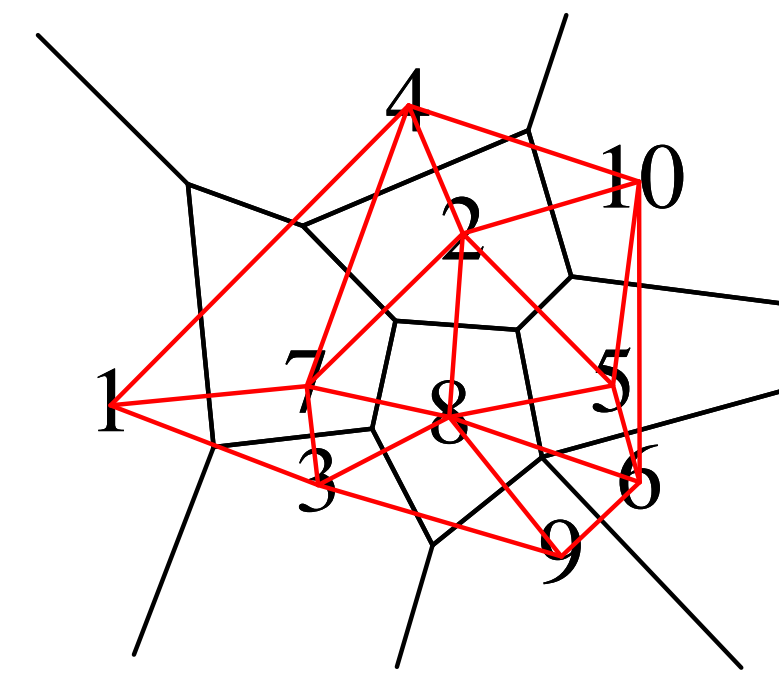
\includegraphics[scale=0.2]{VD_diagram.PNG}
    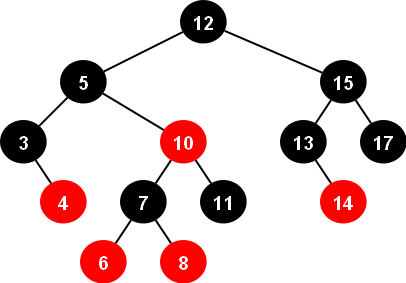
\includegraphics[scale=0.15]{redblacktree.png}
\end{column}
\end{columns}
\begin{itemize}
    \item[]
    \begin{itemize}
        \vspace{-1.15em}
        \item<8-> Dynamic updates and searching in $\ord{\ln(N)}$
        \item<9-> Searches/updates occur $\ord{N}$ times; $\ord{N\ln(N)}$ operations total
    \end{itemize}
    \item<10-> Total time complexity: $\ord{N\ln(N)}$.
\end{itemize}
\end{frame}

\begin{frame}{Complexity of IC-SM}
\alert{A Naïve Cone-Finding Algorithm}
\begin{algorithm}[H]
    \caption{Iterative Cone with Split-Merge}
    \begin{algorithmic}[1]
        \Repeat
            \State $p_t^* \gets \max(\{p_{ti}\})$ \Comment{seed axis}
            \Repeat
                \State $p_j \gets$ sum of momenta of particles within R of seed axis
                \If{$p_t^* == p_j$}
                    \State Label $p_t^*$ a protojet, remove all particles
                \Else
                    \State $p_t^* \gets p_j$
                \EndIf
            \Until{The jet axis and seed axis coincide}
        \Until{No seeds remain}
        \State Run Split-Merge on the protojets
    \end{algorithmic}
\end{algorithm}
\end{frame}

\begin{frame}{Complexity of IC-SM}
\alert{The Split-Merge Procedure}
\begin{algorithm}[H]
    \caption{Split-Merge}
    \begin{algorithmic}[1]
        \State Remove all protojets with $p_t < p_{t,\text{cut}}$
        \Repeat
            \State Determine hardest protojet $i$
            \State Determine hardest protojet $j$ such that $i$ and $j$ share particles
            \If{no such $j$ exists}
                \State $i$ is a final jet; remove particles
            \Else
                \If {$p_{t,\text{shared}} < f\times p_{tj}$}
                    \State Split particles between protojets
                \Else
                    \State Replace $i$ and $j$ with their merger
                \EndIf
            \EndIf
        \Until{no protojets left}
    \end{algorithmic}
\end{algorithm}
\end{frame}

\begin{frame}{Complexity of IC-SM}
\alert{Complexity Analysis}
\begin{itemize}
    \item<2->Stable cone production 
    \begin{itemize}
        \item<3-> Process of finding a stable cone from a seed roughly $\ord{Nn}$ where $n$ is the average particle count in a circle of radius $R$
        \item<4-> This is repeated $\ord{N}$ times.
        \item<5-> Codes MCFM and NLOJet implement this in $\ord{N 2^N}$ by iterating through all possible cones!!
    \end{itemize}
    \item<6-> Split-Merge
    \begin{itemize}
        \item<7-> Determining hardest protojet takes $\ord{N}$
        \item<8-> Finding hardest overlapping jet takes $\ord{N/n}$, repeated $\ord{N}$ times.
        \item<9-> Merging takes $\ord{Nn}$
    \end{itemize}
    \item<10-> Total complexity: $\ord{N^2n}$ (can be optimized to $\ord{N^2}$ with 2D tree data structures)
\end{itemize}
\end{frame}

\begin{frame}{Complexity of SISCone}
\begin{algorithm}[H]
    \caption{SISCone}
    \begin{algorithmic}[1]
        \For{particle i}
            \State Find all particles $j$ within $2R$ of $i$
            \If{no such $j$ exists}
                \State $i$ is made a protojet
            \Else
                \State Find circles of radius $R$ with $i$ $j$ on their circumference
                \For{each circle}
                    \For{each permutations of edge point containment}
                        \State Label circle as cone
                        \State Check cone stability w.r.t the edge points
                    \EndFor
                \EndFor
            \EndIf
        \EndFor
        \State Explicitly check all cones not labeled unstable for stability
    \end{algorithmic}
\end{algorithm}
\end{frame}

\begin{frame}{Complexity of SISCone}
\alert{Improved Cone-Finding}
\begin{figure}
    \centering
    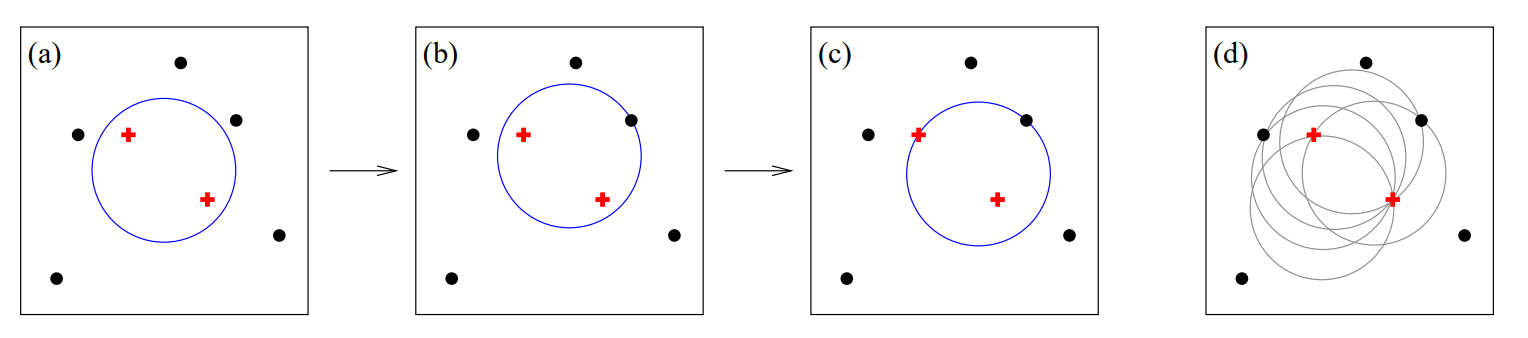
\includegraphics[scale=0.27]{siscone.PNG}
    \caption{SISCone's geometric approach to seedless cone-finding.}
\end{figure}
\begin{itemize}
    \item<2-> SISCone again uses geometric insight to optimize cone finding.
    \item<3-> Able to provably find all stable cones in $\ord{Nn\ln(n)}$ time!
    \item<4-> Seedlessness $\implies$ inherent IR safety
\end{itemize}
\end{frame}

\begin{frame}{Conclusion}
\begin{itemize}
    \item<1-> Jet Reconstruction algorithms are central to modern HEP experiment and theory
    \item<2-> Algorithms need to be fast; algorithmic complexity quantifies this.
    \item<3-> Seemingly the same algorithm can be implement in ways with different complexities
    \begin{itemize}
        \item<4-> $K_t$: $\ord{N^3}$ $\to$ $\ord{N\ln(N)}$
        \item<5-> Cone Algs: $\ord{N2^N}$ $\to$ $\ord{N^3}$ $\to$ $\ord{N^2\ln(N)}$
    \end{itemize}
    \item<6-> We, as physicists, should be embarrassed!
    \begin{itemize}
        \item<7-> (particularly by those $N2^N$ codes...)
    \end{itemize}
    \item<8> Have a good spring break!
\end{itemize}
\end{frame}

\begin{frame}{References}
\begin{thebibliography}{5}
    \bibitem{1} Ryan Atkin 2015 J. Phys.: Conf. Ser. 645 012008
    \bibitem{2} G. P. Salam and G. Soyez, JHEP 0705 (2007) 086 [arXiv:0704.0292 [hep-ph]].
    \bibitem{3} M. Cacciari and G. P. Salam, arXiv:hep-ph/0512210.
    \bibitem{4} S. Fortune, in Proceedings of the second annual symposium on Computational geometry, p. 312 (1986).
\end{thebibliography}
\end{frame}

\end{document}